\chapter{Background}
\label{ch:bg}
In this chapter, we discuss background information and related work for Facet Web Search, an extension of faceted search in the open-domain web setting. Faceted search is a heavily interdisciplinary area, where different aspects of information retrieval, knowledge representation, human computer interaction must be considered all together. Therefore, we first describe related topics in these areas as a background for faceted search/Faceted Web Search. Then, we describe faceted search, Faceted Web Search and previous research on these topics. After that, we discuss related approaches that aim to achieve the same goals as Faced Web Search. We defer discussion of some related work to later chapters where the context makes it more appropriate.

\section{Direct Search and Navigational Search}
Faceted search combines two search paradigms, direct search and navigational search. \textbf{Navigational search} (sometimes also called \concept{directory navigation}) uses a hierarchy structure to enable users to browse the information space by iteratively narrowing the scope of their quest in a predetermined order, as exemplified by Yahoo! Directory\footnote{http://en.wikipedia.org/wiki/Yahoo!\_Directory} and DMOZ\footnote{http://www.dmoz.org/}. Navigational search provides a guided search interface, and supports abstractions that are easily understood by users. However, the strict ordering imposed by the hierarchy structure can be too rigid, especially for large and heterogeneous corpora~\cite{snow2006semantic,tunkelang2009faceted,sacco2009dynamic}. The rapid decline of Yahoo! Directory as a primary web search engine provides pragmatic evidence.

\textbf{Direct search} instead allows users to specify their own queries as input, and is the dominant paradigm in the field of information retrieval. The queries are often keywords in web search scenarios, and thus, sometimes direct search is also called \concept{keyword search}. Direct search resorts to search systems for understanding search intents behind user queries, and returns search results that could best address the search intents. This approach has been made enormously popular by web search engines, such as Google\footnote{http://www.google.com}. However, in the basic search interface, users have to formulate their queries with no or limited assistance, and no exploration capability since results are presented as a flat list with no systematic organization. Faceted search aims to solve this problem, which is described later in Section~\ref{sec:background-fs}. We also discuss other recent advances for addressing this problem in Section~\ref{sec:bg-others}.

\section{Taxonomy and Faceted Taxonomy}
There are two types of information representation (or knowledge representation) related to this work, taxonomies and faceted taxonomies. A \textbf{taxonomy} is an organization of information objects or abstractions into a hierarchy or tree structure~\cite{tunkelang2009faceted}. Navigational search as described above is based on taxonomies. So we have seen two examples of taxonomies, Yahoo! Directory and the Open Directory Project, in which webpages are classified into the hierarchies. An older example is Aristotle's system for organizing knowledge of the human race~\cite{tunkelang2009faceted}. The system classifies living things by dividing them into two groups, plants and animals; further dividing animals into those ``with blood'' and ``without blood''; those with blood into ``live-bearing'' and ``egg-bearing''; and so forth (Figure~\ref{fig:bg-aristotle}).

\begin{figure}[ht!]
\centering
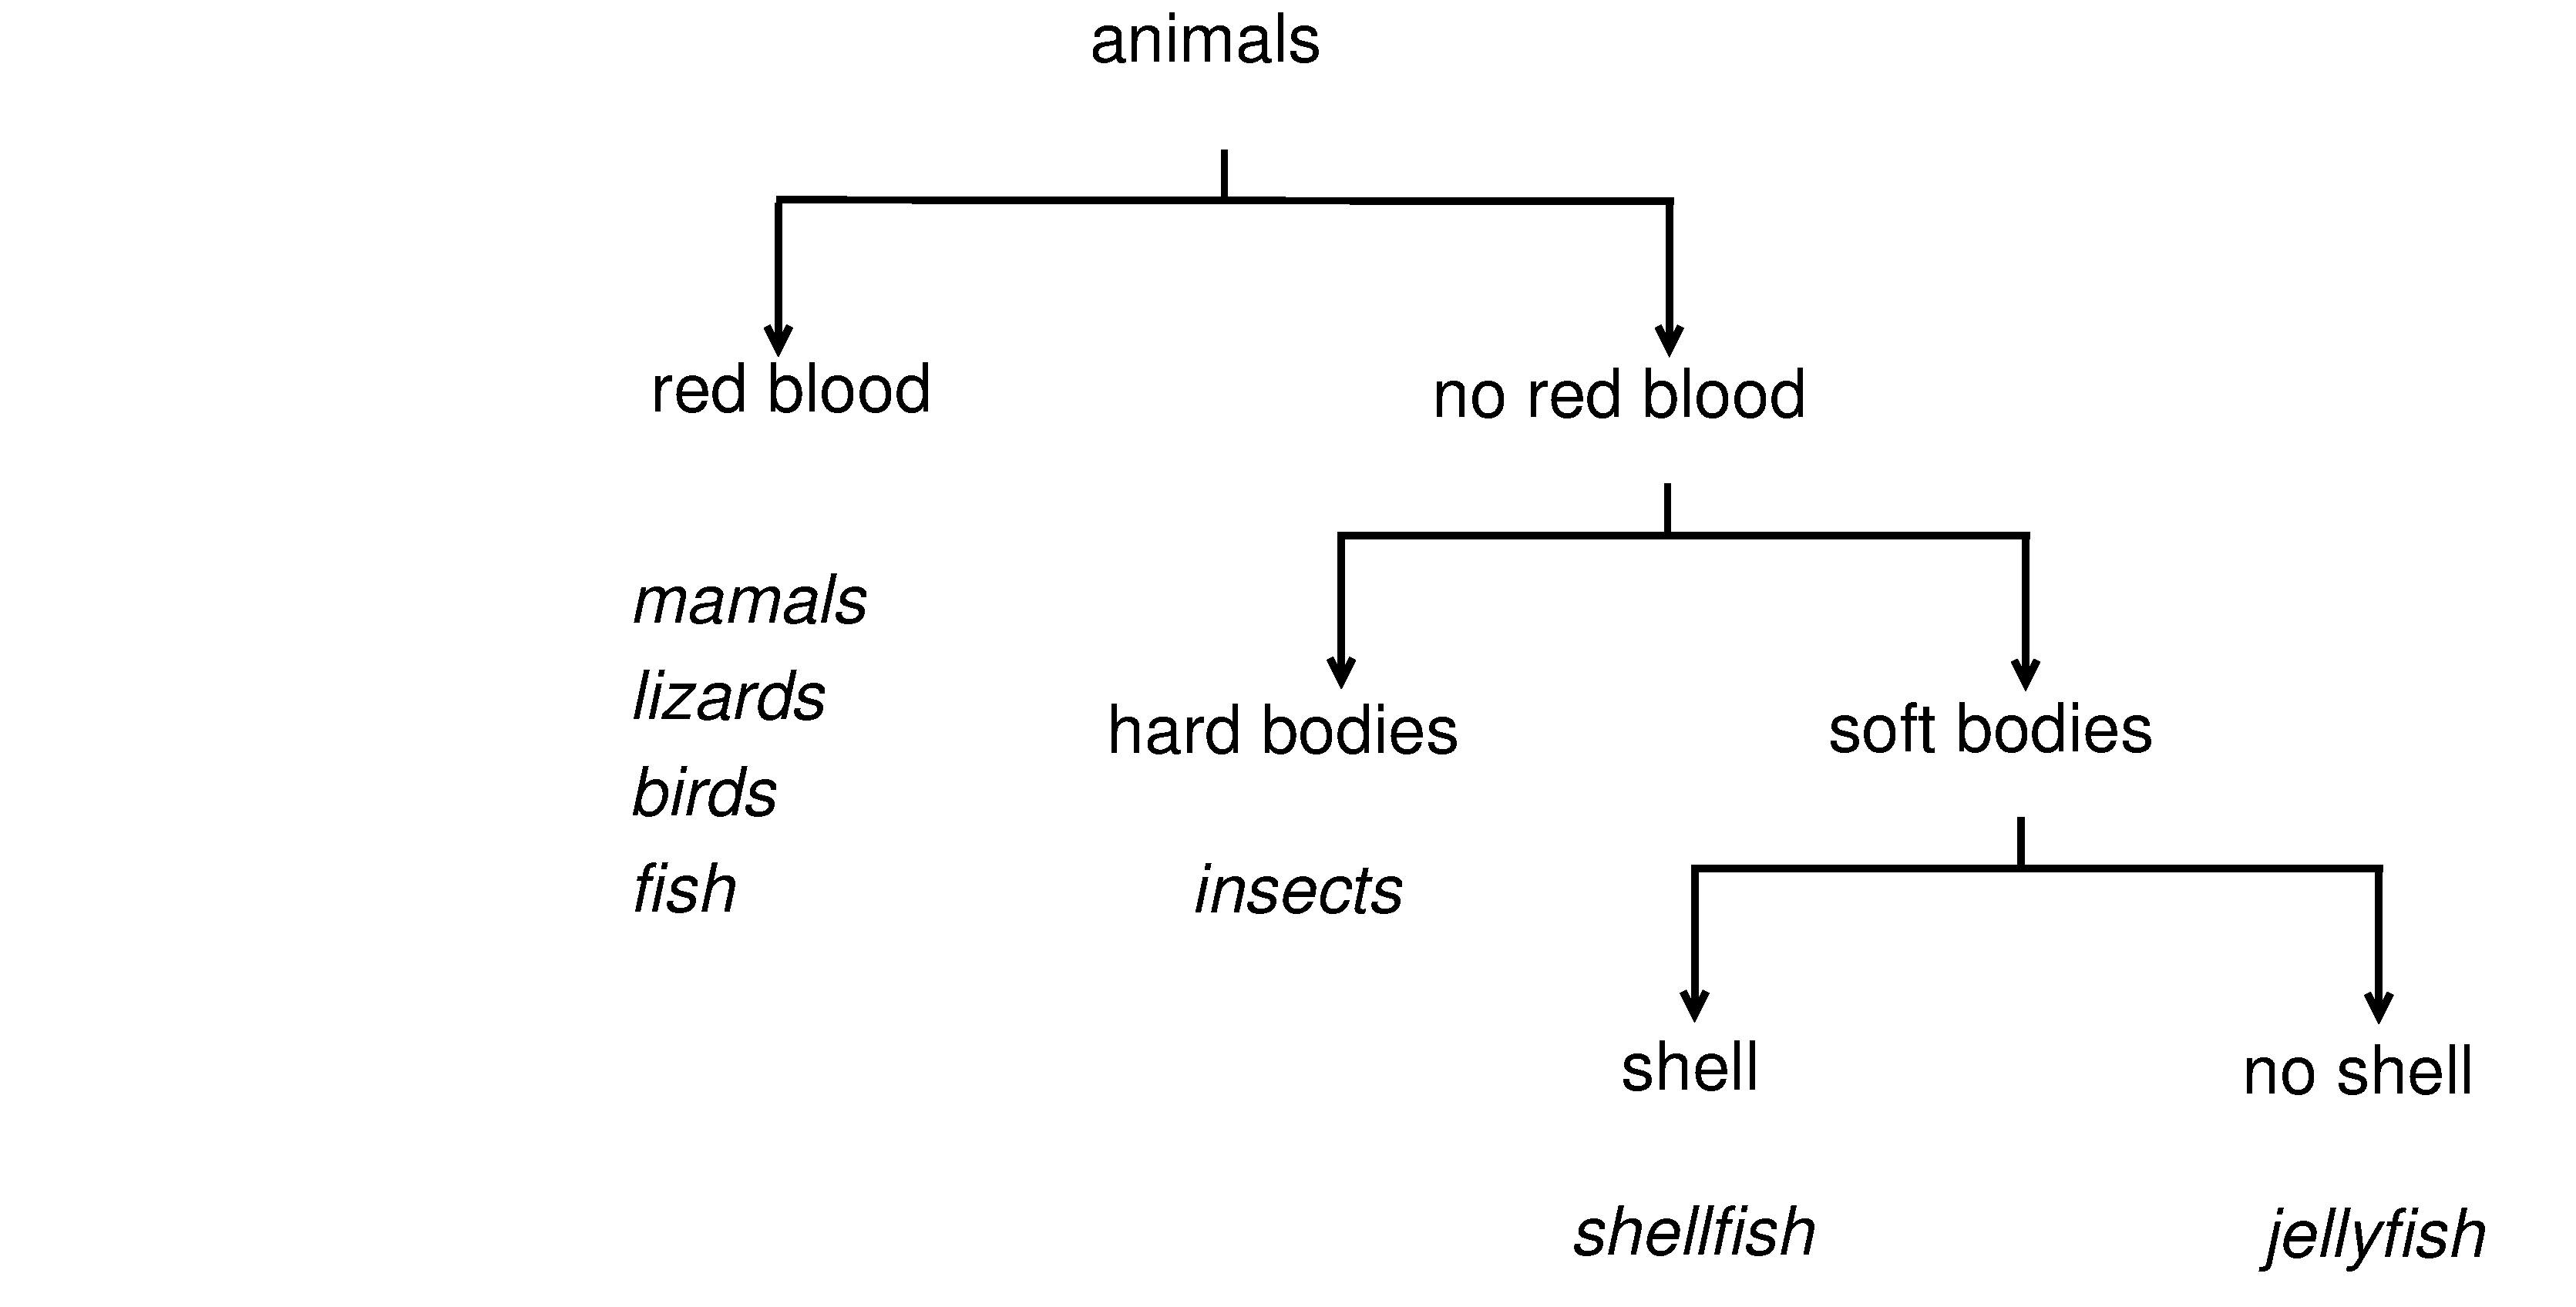
\includegraphics[width=0.95\columnwidth]{drawing/aristotle.eps}
\caption{A subset of Aristotle's knowledge taxonomy~\cite{tunkelang2009faceted}}
\label{fig:bg-aristotle}
\end{figure}

In the context of navigational search, taxonomy enables efficient navigation in the information space. Users start from the root node and iteratively discriminate among children, in order to find the appropriate one. Each time a node is selected for expansion, the total number of objects to be considered is reduced because the objects classified under discarded concepts need not be considered. Thus, users iteratively reduce the number of information objects to be manually inspected~\cite{sacco2009dynamic}.

The key property of a taxonomy is that, for every information object or set of objects that corresponds to a node, there is precisely one unique path to it from the root node. Thus, a taxonomy imposes a strict logical ordering on the information that it represents~\cite{tunkelang2009faceted}. For example, \concept{cancer} can be classified in a taxonomy with a unique path  \concept{disease}$\rightarrow$\concept{structural disease}$\rightarrow$\concept{tumor}$\rightarrow$\concept{cancer}. However, this strict ordering of a taxonomy can be too rigid when dealing with compound information objects. For example, should \concept{treatment of cancer} be a child of \concept{treatment} or of \concept{cancer}? This strict ordering constraint limits expressibility and extensibility of taxonomies and navigational search systems build on them.

Faceted search is based on another type of information representation, called faceted taxonomy, which is sometimes also called multi-dimensional  taxonomy~\cite{sacco2009dynamic} or faceted classification~\cite{tunkelang2009faceted}. A \textbf{faceted taxonomy} is a set of independent taxonomies where each one organizes information objects from a different (preferably orthogonal) point of view, or equivalently based on a different dimension of the multi-dimensional information space. For example, in \textit{Classification, Coding, and Machinery for Search}, \citet{ranganathan1950classification} describe a library system based on a faceted taxonomy for organizing books, with four independent taxonomies mentioned -- the taxonomy \concept{Medicine}, \concept{Disease}, \concept{Treatment} and \concept{Mathematical study}. The four taxonomies each represents one dimension of the multi-dimensional information space for the books. \todo{better example for faceted taxonomy}


The advantage of using multiple independent taxonomies is that they can be combined to describe compound information objects. In Ranganathan's example, the four taxonomies are combined to expresses the topic \concept{statistical study of the treatment of cancer of the soft palate by radium}, as follows. 
\begin{itemize}
 \item Medicine $\rightarrow$ Digestive system $\rightarrow$ Mouth $\rightarrow$ Palate $\rightarrow$ Soft palate
\item Disease $\rightarrow$ Structural disease $\rightarrow$ Tumor $\rightarrow$ Cancer
\item Treatment $\rightarrow$ Treatment by chemical substances $\rightarrow$ Treatment by a chemical element  $\rightarrow$ Treatment by a group 2 chemical element $\rightarrow$ Treatment by radium
\item Mathematical study $\rightarrow$ Algebraical study $\rightarrow$ Statistical study
\end{itemize}
The foci (\concept{Soft palate}, \concept{Cancer}, \concept{Treatment by radium} and \concept{Statistical study}) in each of the taxonomies are combined to express the compound topic, which is difficult in a single hierarchical taxonomy. Combining these independent taxonomies, faceted taxonomies offer expressive power and flexibility beyond single taxonomy used in navigational search. 

%From the example, we can also see that faceted taxonomy enables navigation over , which is called \textbf{faceted navigation}.
Navigation based on a faceted taxonomy is called \textbf{faceted navigation}. In faceted navigation, users can use multiple taxonomies to navigate or explore a multi-dimensional information space. They can narrow the search space by iteratively select child nodes in each of taxonomies. Then the selections on the taxonomy are combined to restrict the matched information objects, as has illustrated in Ranganathan's example. 
\todo{add an example}
\todo{relationships to scatter/gather, clustering}

%pose a challenge for the hierarchical organization of single taxonomies.
\section{Facets}
``Facet'' is a key concept in faceted search. The term \concept{facet} means ``little face'' and is often used to describe one side of a many-sided object, especially a cut gemstone~\cite{teevan2008challenges}. In information science literature, \concept{facet} is a overloaded term. The term has been used to refer both to the entire independent taxonomies in a faceted taxonomy, and to the part of independent taxonomies that are shown to users (as in most of our discussion). In many cases the taxonomies are often shown as shallow or two-level trees. In the computer monitor example (Figure~\ref{fig:intro-amazon}), the facets are two-level (\eg, parent node \concept{Brand} with child nodes \concept{Dell}, \concept{ViewSonic}, \concept{HP}, \concept{Acer}). When there are only two levels in a facet, we can call the parent node (or more precisely, its presentation term) a \textbf{facet label} (\eg, \concept{brand}), and the child nodes \textbf{facet terms} (\eg, \concept{Dell}, \concept{ViewSonic}). It is easy to see that in a two-level facet, facet terms belong to the same semantic class (\ie, the semantic class represented by their parent node). Sometimes, a facet label can be missing or omitted, which results in a one-level facet. So a one-level facet consists of only the facet terms (\eg, \{\concept{Dell}, \concept{ViewSonic}, \concept{HP}, ...\}) with no facet label. This work focuses on studying one-level facets for Faceted Web Search as a start, and leaves the extension of two-level facets to future work.

\todo{exploratory search}

\section{Faceted Search}
\label{sec:background-fs}
\textbf{Faceted Search} combines direct search with faceted navigation, which enables users to navigate a multi-dimensional information space. We have provided an example in Figure~\ref{fig:intro-amazon}. In the example, a user searches with the query \concept{computer monitor} in an e-commercial site, and the site provides the two-level facet \concept{brand}, \concept{display technology} and \concept{condition} for users to select and filter the search results.

Compared with direct search, faceted search provides additional search assistance for users through facets. Facets can assist users in clarifying their search intent and refining the search results (\eg, select \concept{new} in facet \concept{condition} to find only computer monitors in new conditions). Facets also summarize the search space succinctly, and provides exploration suggestions organized in a systematic way (\eg, the listed facet \concept{brand}, \concept{display technology}, \concept{condition} give users an overview of the returned results, and provides them with the key factors they may need to consider when searching for a computer monitor). This exploration capability is especially important in exploratory search tasks, or when users are not exactly clear about what they are looking for~\cite{kules2009exploratory,sacco2009dynamic}.

Compared with navigational search, faceted search supports faceted navigation, which, as outlined above, is especially useful for navigating a multi-faceted information space. In navigational search, the strict ordering imposed by a taxonomy is too rigid when dealing with compound information objects in the multi-faceted information space. Instead, in faceted search, users can combine facets to express complex information need (\eg, \concept{statistical study of the treatment of cancer of the soft palate by radium} in  Ranganathan's example).

\subsection{Automatic Facet Generation}
Previous work on faceted search has studied automatic facet generation ~\cite{dakka2008automatic,li2010facetedpedia,stoica2007automating,oren2006extending,kohlschutter2006using,latha2010afgf} and facet recommendation for a query~\cite{dash2008dynamic,koren2008personalized}. Most of the work is based on existing facet metadata or taxonomies, and extending faceted search to the general web is still an unsolved problem. The challenges stem from the large and heterogeneous nature of the web~\cite{teevan2008challenges}: because the web is very large, it is
difficult to assign quality facets to every document in the collection and to retrieve the full set of search results and their associated facets at query time; and because the web is heterogeneous, it is difficult to apply the same facets to every search result or every query.
%Different from previous work which generates facets for a entire corpus~\cite{stoica2007automating,dakka2008automatic}, some recent work~\cite{dou2011finding,kong2013extracting} extracts facets for only a query.

\subsection{Evaluation for Faceted Search}
Most evaluations for facet generation/recommendation are either based on comparison between system generated and human created facets~\cite{dakka2008automatic,dou2011finding} or user studies~\cite{dash2008dynamic,li2010facetedpedia,stoica2007automating}. However, the former may not exactly reflect the utility of assisting users' search tasks, and the latter is expensive to extend for evaluating new systems. In a spirit similar to ours, some work~\cite{schuth2011evaluation,zhang2010interactive,koren2008personalized} also evaluates facets by their utility in re-ranking documents for users. The differences are their evaluation methods do not capture the time cost for users as explicitly as we do, and their experiments are based on corpora with human created facet metadata. Other evaluations~\cite{burke1996knowledge,english2002hierarchical,hearst2006design,hearst2008uis,kules2009exploratory} for faceted search are mostly done from a user interface perspective, which is beyond the scope of 
this proposal.

\section{Other Related Techniques}
\label{sec:bg-others}
A number of other areas are similar in spirit to ours, We discuss query subtopic mining, semantic class extraction, search result diversification and search result clustering/organization.
\subsection{Query Subtopic/Aspect Mining}
To address multi-faceted queries, much previous work studied mining query subtopics (or aspects). 
A query subtopic is often defined as a distinct information need relevant to the original query.
It can be represented as a set of terms that together describe the distinct information need~\cite{wang2009mining,wu2011identifying, dang2011inferring} or as a single keyword that succinctly describes the topic~\cite{song2011overview}. 
Different resources have been used for mining query subtopics, including query logs~\cite{wang2007learn,hu2012mining,xue2011topic,wang2009mining,wu2011identifying,yin2010building}, document corpus~\cite{allan2002using} and anchor texts~\cite{dang2011inferring}.
\todo{top-ranked docs?}
% Much work~\cite{Wang:2007:LWS:1277741.1277759, Hu:2012:MQS:2348283.2348327} uses related queries from search logs as candidates, and clustered them into query subtopics. Wang and Zhai~\cite{Wang:2007:LWS:1277741.1277759}, for example, used snippets of a query's clicked web documents to enrich the query representation, and then cluster related past queries into query subtopics.
%Due to data sparsity for instance-level query subtopics, Some work~\cite{Wang:2009:MBL:1557019.1557114,Xue:2011:TMN:2063576.2063877,Wu:2011:IAW:2016945.2016963,Yin:2010:BTW:1772690.1772792} mined generic query subtopics, which are query subtopics for a generic class of queries.
%For example, Yin et al.~\cite{Yin:2010:BTW:1772690.1772792} built taxonomies of query subtopics for categories of name entity queries using search logs.
%Wu et al.~\cite{Wu:2011:IAW:2016945.2016963} also worked on identifying query aspects for named entities queries. They propagated reformulation phrases for a classes of named entities queries.
%Other than query logs, query subtopics can also be mined from documents. For example, Dang et al.~\cite{Dang:2011:IQA:2063576.2063904} worked on clustering related anchor texts in ClueWeb09 corpus into query subtopics. Allan et al.~\cite{Allan:2002:UPP:564376.564430}, from a text corpus, extracted commonly occurring parts of speech pattern near a single-word query to find different potential specifications of the query.


Query subtopics and facets for a query are different in that the terms in a query subtopic are not restricted to be coordinate terms, or to have peer relationships. Facets for a query, however, organize terms by grouping ``sibling'' terms together. For example, \{\textit{news}, \textit{cnn}, \textit{latest news}, \textit{mars curiosity news}\} is a valid query subtopic for the query \textit{mars landing}, which describes the search intent of Mars landing news, but it is not a valid facet. Instead, a valid facet that describes Mars landing news could be \{\textit{cnn}, \textit{abc}, \textit{fox}\}, which includes different news channels.
%In a recent work~\cite{Dou:2011:FDQ:2063576.2063767}, Dou et al. developed a system to extract facets from web search results and showed the potential of doing so. However, the unsupervised method they proposed is far from optimal, and it does not improve by having human labels available. Also, to the best of our knowledge, their evaluation can be problematic in some cases, which will be discussed in Section~\ref{sec:evalmetricsall}.

\subsection{Semantic Class Extraction}
Semantic class extraction is to automatically mine semantic classes represented as their class instances from certain data corpora. For example, it may extract \textit{USA}, \textit{UK}, \textit{China} as class instances of semantic class \textit{country}. Due to the similar semantic relationships between terms inside a facet and a semantic class, semantic class extraction can be used for facet generation. Existing approaches can be roughly divided into two categories: distributional similarity and pattern-based~\cite{shi2010corpus}. The distributional similarity approach is based on the distributional hypothesis~\cite{Harris}, that terms occurring in analogous contexts tend to be similar. Different types of contexts have been studied for this problem, including syntactic context~\cite{pantel2002discovering} and lexical context~\cite{pantel2004towards,agirre2009study,pantel2009web}.
The pattern-based approach applies textual patterns~\cite{hearst1992automatic,pasca2004acquisition}, HTML patterns~\cite{shinzato2007simple} or both~\cite{zhang2009employing,shi2010corpus} to extract instances of a semantic class from some corpus.
The raw semantic class extracted can be noisy. To address this problem, \citet{zhang2009employing} used topic modeling to refine the extracted semantic classes.
Their assumption is that, like documents in the conventional setting, raw semantic classes are generated by a mixture of hidden semantic classes.\todo{describe similarity}
In this work, we apply pattern-based semantic class extraction on the top-ranked Web documents to extract candidates for query facet generation.

\subsection{Search Results Diversification}
Search result diversification has been studied as a method of tackling ambiguous or multi-faceted queries while a ranked list of documents remains the primary output feature of Web search engine today~\cite{agrawal2009diversifying,clarke2008novelty,santos2010exploiting,sakai2011evaluating,dang2013term}.
The purpose is to diversify the ranked list to account for different search intents or query subtopics.
A weakness of search result diversification is that the query subtopics are hidden from the user, leaving him or her to guess at how the results are organized.
FWS addresses this problem by explicitly presenting different facets of a query using groups of coordinate terms for users to select.
\todo{difference}

\subsection{Search Result Clustering/Organization}
Search results clustering is a technique that tries to organize search results by grouping them into, usually labeled, clusters by query subtopics~\cite{carpineto2009survey}.\todo{change citation}
It offers a complementary view to the flat ranked list of search results.
Most previous work has exploited different textual features extracted from the input texts and applied different clustering algorithms with them.

Instead of organizing search results in groups, there is also some work~\cite{lawrie2001finding,lawrie2003generating, nevill1999lexically} that summarizes search results or a collection of documents in a topic hierarchy. For example, previous studies~\cite{lawrie2001finding,lawrie2003generating} used a probabilistic model for creating topical hierarchies, in which a graph is constructed based on conditional probabilities of words, and the topic words are found by approximately maximizing the predictive power and coverage of the vocabulary. \todo{similar to taxonomy}

FWS is different from these work in that it provides facets of a query, instead of directly organizing the search results. The facet interface allows users to filter/re-rank search results from multiple aspects, instead of a single, taxonomic order.

%\section{User Feedback}
%There is a long history of using user explicit feedback to improve retrieval performance. In relevance feedback~\cite{rocchio71relevance,salton90improvingretrieval}, documents are presented to users for judgment, after which terms are extracted from the judged relevant document, and added into the retrieval model. In the case where true relevance judgments are unavailable, top documents are assumed to be relevant, which is called pseudo relevance feedback~\cite{buckley1995automatic,abdul2004umass}. Because a document is a large text unit which can be difficult for users to judge and for the system to incorporate relevance information, previous work also studied user feedback on passages~\cite{allan1995relevance,xu1996query} and terms~\cite{koenemann1996case,tan2007term}.

%For faceted search, previous work~\cite{zhang2010interactive} studied user feedback on facets, using both boolean filtering and soft ranking models. However, the study is based on corpora with human created facet metadata, which is difficult to obtain for the general web. One other difference between our work and most other user feedback work is, facet feedback in our work is used to improve ranking with respect to the query subtopic specified by the feedback terms, instead of the query topic represented by the original query. This presents the scenario in FWS, where users start with a less-specified query, and then use facets to help clarify and search for subtopic information.

\section{Summary}
\todo{re-state facet and facet term definition here}
Faceted web search (FWS) we propose in this work is different from all the past work. It extends conventional faceted search from a fixed-domain setting to an open-domain web setting. It is different from search result diversification in that instead of hiding those query subtopics from users, it explicitly presents different facets of a query. It is also different from search results clustering or organization in that instead of directly organizing the search results, the facet interface in FWS allows users to filter/re-rank search results from multiple aspects.

We study three main issues of FWS that have not been explored in previous work, including facet generation, facet feedback and evaluation for FWS. Facet generation for FWS is different from query subtopic mining due to the different nature of query subtopics and facets. It is also different from semantic class extraction in that it targets a general web query instead of a semantic class. Facet feedback for FWS is different from other user feedback due to their different purposes. Facet feedback targets at improving ranking with respect to the ``query subtopic'' specified by the feedback terms, instead of the query topic represented by the original query. Our evaluation for FWS is also different from previous ones for faceted search. We consider many different aspects (e.g., cost and gain), and the evaluation is based on simulations instead of user studies, which makes it relative cheap to extend for new systems. \todo{the evaluation description is not in this chapter}
